%%%%%%%%%%%%%%%%%%%%%%%%%%%%%%%%%%%%%%%%%%%%%%%%%%%%%%%%%%%%%%%%%%%%%%%%%%%%%%%%
% IEEE Conference Template for CSE356 IoT Project
% - Structured for the 10-step IoT Design Methodology
% - Configured for BibTeX (references.bib) and a figures folder
%%%%%%%%%%%%%%%%%%%%%%%%%%%%%%%%%%%%%%%%%%%%%%%%%%%%%%%%%%%%%%%%%%%%%%%%%%%%%%%%

\documentclass[conference]{IEEEtran}
\IEEEoverridecommandlockouts
% The preceding line is only needed to identify funding in the first footnote. If that is unneeded, please comment it out.
% \usepackage{cite}
\usepackage{booktabs}
\usepackage{amsmath,amssymb,amsfonts}
\usepackage{algorithmic}
\usepackage{graphicx}
\usepackage{caption}
\usepackage{textcomp}
\usepackage{xcolor}
\usepackage{tabularx}
\usepackage{float}
\usepackage{placeins}

\def\BibTeX{{\rm B\kern-.05em{\sc i\kern-.025em b}\kern-.08em
    T\kern-.1667em\lower.7ex\hbox{E}\kern-.125emX}}

% Set the path for your figures directory
\graphicspath{{figures/}}

\usepackage{tikz}
\usetikzlibrary{fit}
\usetikzlibrary{arrows.meta,positioning,shadows.blur}

\definecolor{primary}{HTML}{0A84FF}
\definecolor{accent}{HTML}{FF453A}
\definecolor{ink}{HTML}{0A0A0A}

\begin{document}

% --- TITLE ---
\title{Design and Prototyping of an IoT Smart Home Security System\\
}

% --- TEAM'S NAMES ---
\author{\IEEEauthorblockN{Hamsa Ahmad}
\IEEEauthorblockA{\textit{Computer and Systems Eng. Dept.} \\
\textit{Ain Shams University}\\
Cairo, Egypt \\
20P1874@eng.asu.edu.eg}
\and
\IEEEauthorblockN{Ahmad Muhammad Abdelmaksoud}
\IEEEauthorblockA{\textit{Computer and Systems Eng. Dept.} \\
\textit{Ain Shams University}\\
Cairo, Egypt \\
2101077@eng.asu.edu.eg}
\and
\IEEEauthorblockN{Salma Mohamed Yousef}
\IEEEauthorblockA{\textit{Computer and Systems Eng. Dept.} \\
\textit{Ain Shams University}\\
Cairo, Egypt \\
21P0148@eng.asu.edu.eg}
\and
\IEEEauthorblockN{Adham Osama Mohamed Nour}
\IEEEauthorblockA{\textit{Computer and Systems Eng. Dept.} \\
\textit{Ain Shams University}\\
Cairo, Egypt \\
22p0071@eng.asu.edu.eg}
\and
\IEEEauthorblockN{Belal Anas Awad}
\IEEEauthorblockA{\textit{Computer and Systems Eng. Dept.} \\
\textit{Ain Shams University}\\
Cairo, Egypt \\
21P0072@eng.asu.edu.eg}
}

\maketitle

% --- ABSTRACT AND KEYWORDS ---
\begin{abstract}
This paper presents the complete 10-step design methodology for an IoT-based Smart Home Security System. The system is designed to detect unauthorized access through a network of sensors, capture evidence using cameras, and provide real-time alerts to the homeowner. The design covers all aspects from requirement analysis and system modeling to the specification of devices, services, and applications, culminating in a comprehensive blueprint for implementation and simulation.
\end{abstract}

\begin{IEEEkeywords}
Internet of Things, IoT, Smart Home, Security System, System Design, Cisco Packet Tracer
\end{IEEEkeywords}


%%%%%%%%%%%%%%%%%%%%%%%%%%%%%%%%%%%%%%%%%%%%%%%%%%%%%%%%%%%%%%%%%%%%%%%%%%%%%%%%
% --- START OF THE PROJECT REPORT BODY ---
%%%%%%%%%%%%%%%%%%%%%%%%%%%%%%%%%%%%%%%%%%%%%%%%%%%%%%%%%%%%%%%%%%%%%%%%%%%%%%%%

\section{Introduction}

The Internet of Things (IoT) has emerged as a transformative technology, connecting everyday objects to the internet and enabling intelligent automation and monitoring\cite{startertutorials_IoT_methodology, achtaich2021guidelines, seerangan_domain_specific_iot_home_automation_2022, article_S266729522100026X}. One of the most impactful applications of IoT is in the domain of smart home systems, where connected devices enhance convenience, energy efficiency, and security \cite{yamini_home_intrusion_2016, design_implementation_smart_home_IoT_2024, sharma_iot_based_smart_home_automation_2020, zwemer_smart_home_iot_part2_2015}. Home security, in particular, has seen significant innovation through IoT, moving from traditional isolated alarm systems to interconnected, responsive networks that provide homeowners with real-time awareness and control\cite{tipirisetty_home_automation_case_study_2025, startertutorials_IoT_methodology}.

This paper details the design of an IoT-based Smart Home Security System. The primary objective is to create a robust and reliable system that detects potential intrusions and promptly alerts the homeowner. To ensure a thorough and systematic design, we adhere to the 10-step IoT design methodology \cite{seerangan_domain_specific_iot_home_automation_2022}, covering all aspects from initial requirements to application development.The following sections will elaborate on each step of this methodology, providing a complete blueprint for the system's architecture and functionality.


\section{IoT System Design Methodology}
This section details the design of the Smart Home Security System following the prescribed 10-step methodology.

% --- STEP 1 ---
\subsection{Step 1: Purpose \& Requirements Specification}
The primary purpose of this IoT system is to enhance home security by providing real-time detection of unauthorized entry or suspicious activity and notifying homeowners immediately \cite{yamini_home_intrusion_2016, achtaich2021guidelines, seerangan_domain_specific_iot_home_automation_2022}. This system aims to be a proactive deterrent and a reliable monitoring tool, offering peace of mind to the user by integrating physical sensors with a smart notification platform.
\subsubsection{\textbf{Functional Requirements:}}
Functional requirements such as door/window monitoring, motion sensing, and camera integration follow standards highlighted in both recent specifications and case studies \cite{wang_iot_devices_security_2024, design_implementation_smart_home_IoT_2024}.
\begin{itemize}
    \item \textbf{Door/Window Monitoring:} The system must use magnetic sensors to detect when a door or window is opened and register this as a potential intrusion event.
    \item \textbf{Motion Detection:} PIR motion sensors must be able to detect human movement within designated areas of the home.
    \item \textbf{Camera Integration:} The system must be able to trigger a camera to capture images or video footage upon detecting a security event (e.g., a door opening or motion).
    \item \textbf{Real-time Alerts:} The system must send immediate notifications (e.g., push notifications or SMS) to the homeowner's mobile application when an event is detected.
    \item \textbf{Remote Control:} The homeowner must have the ability to arm or disarm the system and remotely control connected devices, such as activating a siren or turning on lights.
    \item \textbf{Monitoring Dashboard:} The mobile application must provide a live view of all sensor statuses and a log of past events.
\end{itemize}
\subsubsection{\textbf{Non-Functional Requirements:}}Non-functional requirements, such as reliability, secure communication, scalability, and energy efficiency, are informed by IETF drafts and smart device standards \cite{wang_iot_devices_security_2024}.
\begin{itemize}
    \item \textbf{High Reliability:} The system must be highly reliable with a low rate of false alarms to maintain user trust.
    \item \textbf{Secure Communication:} All data transmission between sensors, the IoT hub, and the cloud must be encrypted to prevent eavesdropping or tampering.
    \item \textbf{Scalability}: The system must be designed to easily accommodate additional sensors, cameras, and other devices as the user’s needs grow.
    \item \textbf{Energy Efficiency:} Battery-powered sensors must have a long lifespan, minimizing the need for frequent battery replacement.
    \item \textbf{Low Latency:} The time from event detection to notification delivery must be as short as possible, ideally less than two seconds.
\end{itemize}


% --- STEP 2 ---
\subsection{Step 2: Process Specification}
% --- Person 1 (SALMA) writes here ---
% Describe the main processes of the system (e.g., intrusion detection, alerting).
% You can add a flowchart figure here later.
The core process of the system involves a continuous cycle of sensing, processing, and reacting. This process is initiated by a physical event and culminates in a user notification and, potentially, an automated action\cite{startertutorials_IoT_methodology, cisco_packettracer_iot}.
\begin{itemize}
    \item \textbf{Event Detection}: The process begins when a sensor is triggered. A magnetic sensor detects the state change from a closed door to an open door, or a PIR sensor detects a change in infrared radiation, indicating movement.
    \item \textbf{Data Transmission:} The triggered sensor sends a wireless signal (e.g., via Zigbee or Wi-Fi) containing event data (e.g., "door\_sensor\_1: open") to the central IoT hub.
    \item \textbf{Hub-side Processing:} The IoT hub receives the data and performs a preliminary check. If the system is armed, it determines that this event requires further action.
    \item \textbf{Cloud Communication:} The hub forwards the event data to a cloud-based backend. This data is packaged as a lightweight message (e.g., JSON payload via MQTT).
    \item \textbf{Cloud-side Analysis \& Action:} The cloud server performs several critical functions.
    \item \textbf{Event Classification:} It analyzes the event data to confirm it's a valid intrusion alert.
    \item \textbf{Notification Generation:} It generates a push notification or other form of alert, containing relevant details like the sensor ID and timestamp.
    \item \textbf{Command Triggering:} It sends a command back to the IoT hub to trigger a connected actuator, such as activating a siren or a smart camera to start recording.
    \item \textbf{User Notification:} The notification is delivered to the homeowner's mobile application.
    \item \textbf{User Interaction:} The user can interact with the app to view the event log, review camera footage, or remotely disarm the system.
\end{itemize}



% --- STEP 3 ---
\subsection{Step 3: Domain Model Specification}
The domain model specifies the main entities of the Smart Home Security System and
the relationships between them. It provides a conceptual blueprint of how different
components interact within the system \cite{achtaich2021guidelines, seerangan_domain_specific_iot_home_automation_2022, zwemer_smart_home_iot_part2_2015}.

\subsubsection{Entities}
\begin{itemize}
    \item \textbf{Homeowner:} The end user who interacts with the system through the mobile application to monitor, control, and receive alerts.
    \item \textbf{Sensors:} Include magnetic door/window sensors and PIR motion sensors. They generate raw event data such as ``open/closed'' or ``motion detected''.
    \item \textbf{Cameras:} Capture images or video footage when triggered by intrusion events or homeowner commands.
    \item \textbf{Zones:} Logical groupings of sensors and cameras (e.g., Living Room, Main Entrance) used to organize monitoring and reporting.
    \item \textbf{Events:} Represent occurrences detected by the system, categorized by type (e.g., door open, motion) and linked to specific devices and timestamps.
    \item \textbf{Notifications:} User-facing alerts generated by the system and delivered via the mobile app.
    \item \textbf{IoT Hub/Gateway:} Collects data from sensors and cameras, performs initial checks, and forwards relevant information to the cloud.
    \item \textbf{Cloud Backend:} Processes and classifies data, stores event logs and media, and generates notifications.
    \item \textbf{Mobile Application:} Provides the user interface for real-time alerts, device status, live video streams, and remote control.
\end{itemize}

\subsubsection{Relationships}
\begin{itemize}
    \item Sensors and Cameras send data to the IoT Hub.
    \item The IoT Hub forwards data to the Cloud for processing and storage.
    \item The Cloud generates alerts and notifications, which are sent to the Mobile Application.
    \item The Homeowner interacts with the Mobile Application to monitor and control the system.
    \item The Mobile Application can trigger camera actions or send control commands back through the Cloud to the IoT Hub.
\end{itemize}

\subsubsection{Domain Model Diagram}
\begin{figure}[htbp]
\centerline{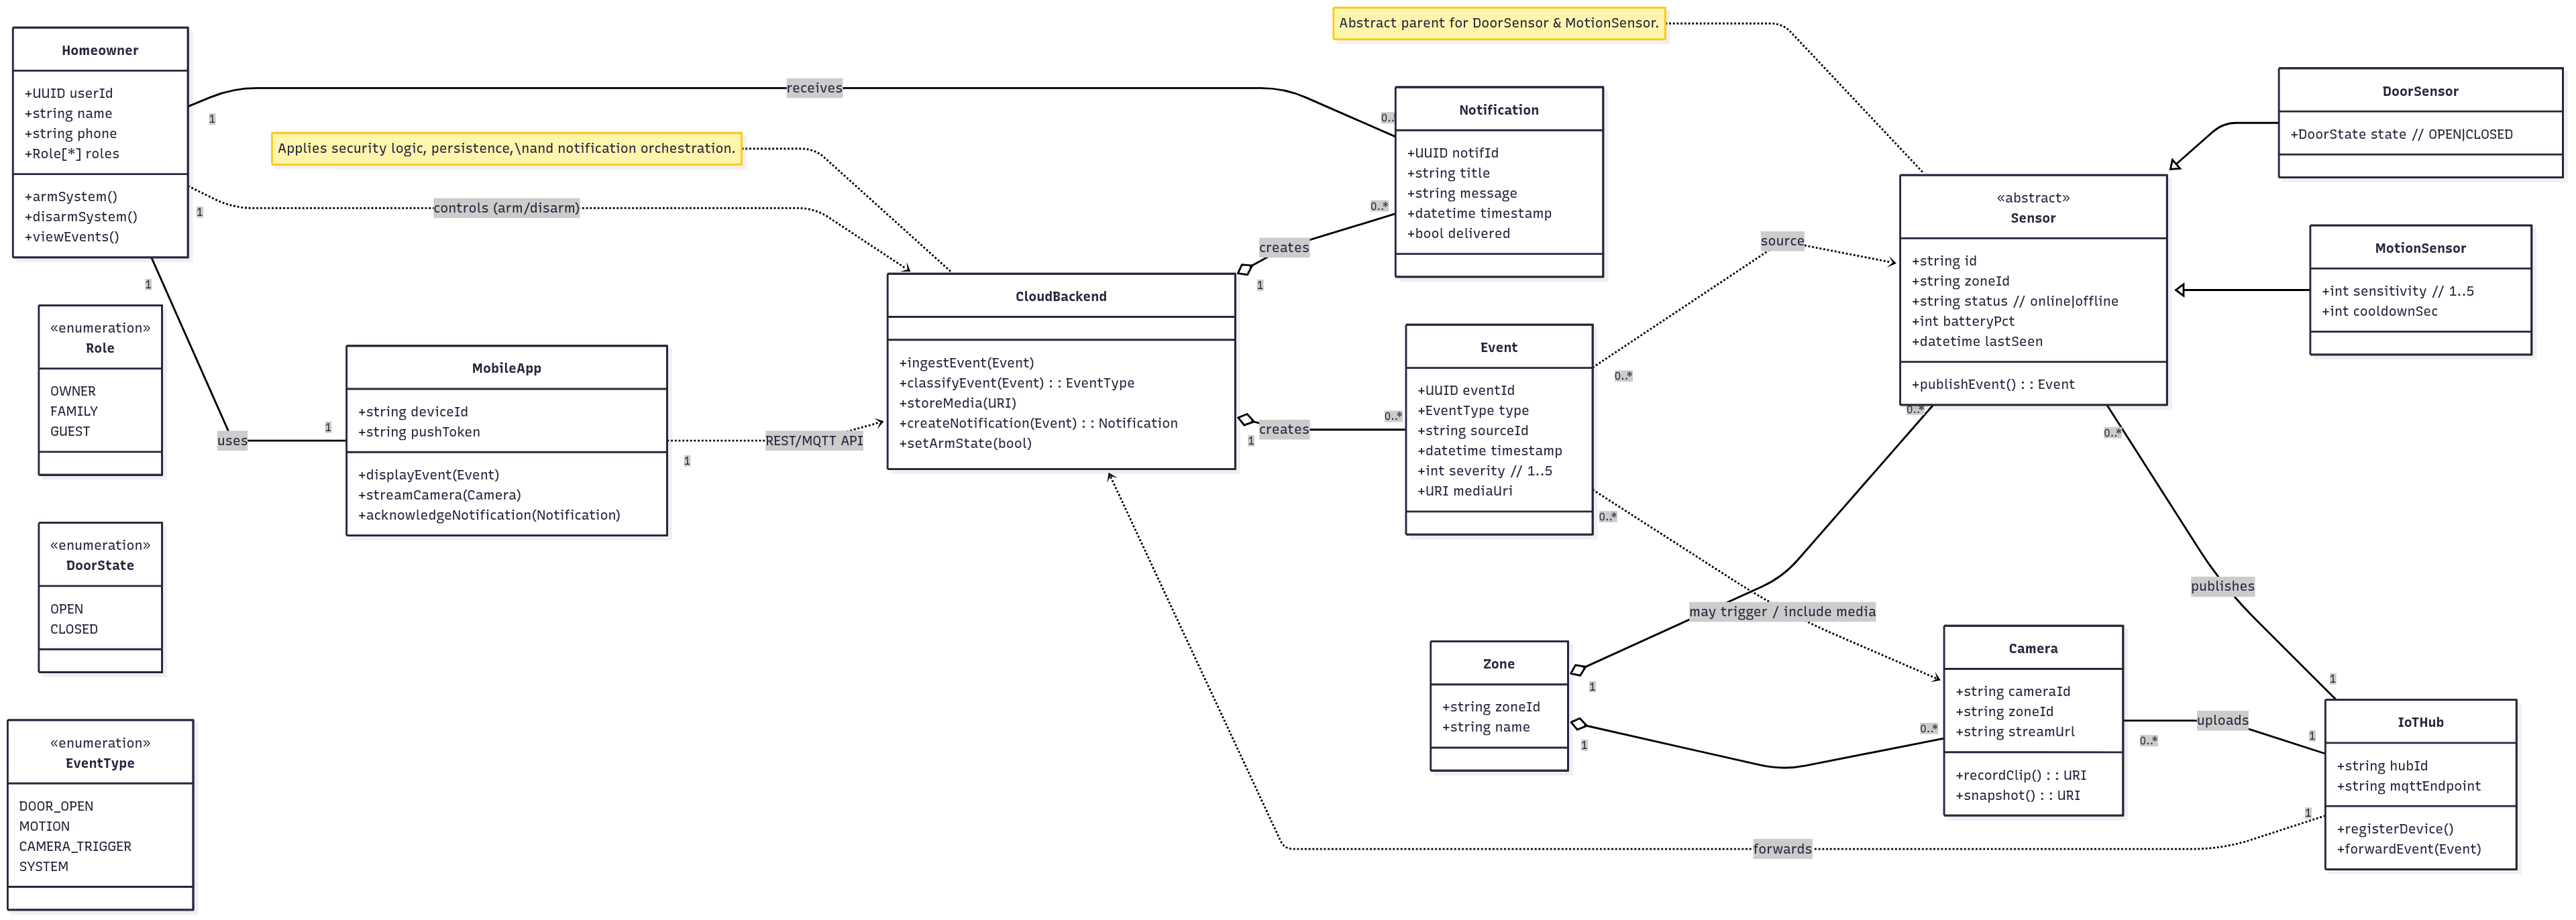
\includegraphics[width=0.9\columnwidth]{domain_model.png}}
\caption{Domain model (UML Class Diagram) showing entities, relationships, and interactions in the Smart Home Security System.}
\label{fig:domain-model}
\end{figure}



% --- STEP 4 ---
\subsection{Step 4: Information Model Specification}
% --- Person 2 (AHMED) writes here ---
% A. Specify the data generated by each component (e.g., sensor status, video stream).
% B. Detail the structure and flow of information through the system.
The information model defines the data elements used, generated, and exchanged within the Smart Home Security System. It ensures consistency in how information flows across devices, the IoT hub, the cloud, and the user application \cite{wang_iot_devices_security_2024, article_S266729522100026X}.

\subsubsection{Data Generated by Components}
\begin{itemize}
    \item \textbf{Door/Window Sensor:} Produces a binary status (\texttt{0 = Closed, 1 = Open}) along with a unique sensor ID and timestamp.
    \item \textbf{PIR Motion Sensor:} Outputs a boolean flag (\texttt{0 = No Motion, 1 = Motion Detected}), sensor ID, and timestamp.
    \item \textbf{Camera:} Captures multimedia data in the form of still images (JPEG) or video clips (MP4), triggered by intrusion events or user commands. Metadata includes camera ID, timestamp, and event reference.
    \item \textbf{IoT Hub/Gateway:} Aggregates sensor data, packages it into lightweight payloads (e.g., JSON objects), and attaches zone identifiers before forwarding to the cloud.
    \item \textbf{Cloud Backend:} Applies intrusion detection logic (armed/disarmed state, event correlation), classifies incoming events, stores structured logs in a database (sensor ID, event type, timestamp, zone, status), and manages large unstructured data (image/video) in secure object storage.
    \item \textbf{Notifications:} JSON payloads generated by the Cloud Backend and delivered to the Mobile Application, containing event type, device ID, zone, and timestamp.
    \item \textbf{Mobile Application:} Receives notifications, displays device status, and requests historical logs or media from the cloud.
\end{itemize}

\subsubsection{Information Flow}
The system’s data pipeline follows a structured flow: 
\begin{enumerate}
    \item Sensors capture physical events (open/close, motion).
    \item Data is transmitted wirelessly (Zigbee/Wi-Fi) to the IoT hub.
    \item The hub standardizes the data into JSON messages and forwards it to the cloud.
    \item The cloud applies intrusion-detection logic, analyzes and classifies the data, storing structured logs in databases and media in cloud storage.
    \item Notifications are generated as JSON messages and pushed to the homeowner’s mobile application.
    \item The user interacts with the app to request live feeds or historical logs, which are retrieved from the cloud on demand.
\end{enumerate}

\subsubsection{Example Data Structures}
\begin{itemize}
    \item \textbf{Door Sensor Event (JSON):}
\begin{verbatim}
{
  "device_id": "door_01",
  "zone": "main_entrance",
  "status": "open",
  "timestamp": "2025-08-28T19:45:00Z"
}
\end{verbatim}

    \item \textbf{Motion Sensor Event (JSON):}
\begin{verbatim}
{
  "device_id": "motion_03",
  "zone": "living_room",
  "motion": true,
  "timestamp": "2025-08-28T19:46:10Z"
}
\end{verbatim}

    \item \textbf{Notification Payload (JSON):}
\begin{verbatim}
{
  "event_type": "intrusion_detected",
  "device_id": "motion_03",
  "zone": "living_room",
  "timestamp": "2025-08-28T19:46:10Z",
  "action": "view_camera"
}
\end{verbatim}
\end{itemize}


\subsubsection{Information Model Diagram}

\begin{center}
% 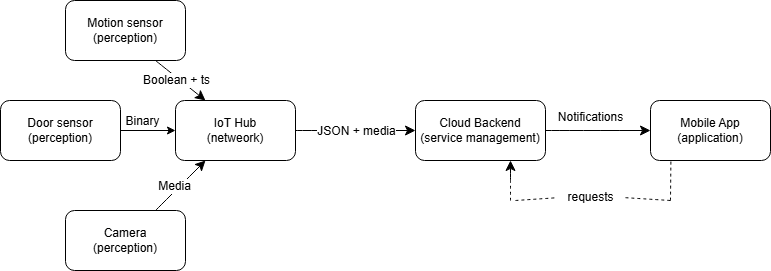
\includegraphics[width=\columnwidth]{information_model.png}
\centerline{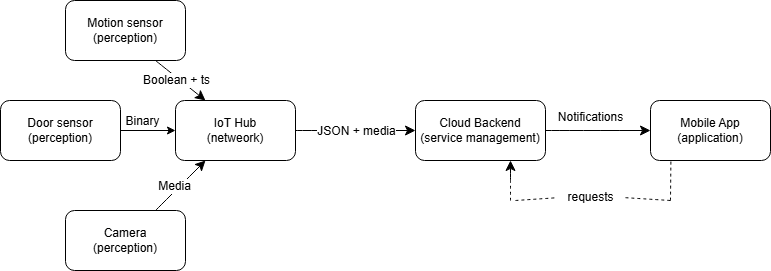
\includegraphics[width=0.9\columnwidth]{information_model.png}}


\captionof{figure}{Information model showing sensor data flow (binary, boolean, media) through the IoT Hub and Cloud Backend to the Mobile App, with dashed arrows for user and actuator commands.}
\label{fig:information-model}
\end{center}

% --- STEP 5 ---
\subsection{Step 5: Service Specifications}
The service specifications define the logical services offered by the IoT system \cite{design_implementation_smart_home_IoT_2024}. These services represent the core functionalities and are exposed through well-defined interfaces (e.g., REST APIs, MQTT topics) that allow different components of the system to interact. These services are primarily hosted and executed within the cloud backend (Level 3)\cite{tipirisetty_home_automation_case_study_2025, startertutorials_IoT_methodology, sharma_iot_based_smart_home_automation_2020}.

\subsubsection{Intrusion Detection Service}
This is the central logic service responsible for analyzing incoming events and determining if a security threat exists.
\begin{itemize}
    \item \textbf{Description:} It consumes sensor data, correlates it with the system's current state (e.g., Armed/Disarmed), and applies predefined security rules to identify potential intrusions.
    \item \textbf{Interface:} Consumes messages from an MQTT topic.
    \item \textbf{Operations:}
    \begin{itemize}
        \item \texttt{ProcessSensorEvent}: Triggered when a new message arrives on the \texttt{/home/events/raw} topic. It takes a JSON payload from a sensor as input, evaluates it, and triggers other services (Notification, Event History) upon detecting a valid intrusion.
    \end{itemize}
\end{itemize}

\subsubsection{Notification Service}
This service is dedicated to delivering real-time alerts to the homeowner.
\begin{itemize}
    \item \textbf{Description:} It formats and dispatches notifications through various channels based on user preferences.
    \item \textbf{Interface:} Internal service-to-service API, invoked by the Intrusion Detection Service.
    \item \textbf{Operations:}
    \begin{itemize}
        \item \texttt{SendAlert(UserID, EventData)}: Takes a target user and event details as input. It then pushes a formatted message to the appropriate platform notification service (e.g., Apple Push Notification Service, Firebase Cloud Messaging).
    \end{itemize}
\end{itemize}

\subsubsection{Event History Service}
This service provides data persistence for all security-related events, enabling historical review.
\begin{itemize}
    \item \textbf{Description:} It logs all events detected by the system and provides an interface for the mobile application to query this history.
    \item \textbf{Interface:} Internal event logging and a public RESTful API for data retrieval.
    \item \textbf{Operations:}
    \begin{itemize}
        \item \texttt{LogEvent(EventData)}: An internal operation triggered by the Intrusion Detection Service to write an event to the database.
        \item \texttt{GET /api/events}: A REST API endpoint for the mobile app to fetch a list of historical events. It supports query parameters for filtering (e.g., \texttt{?zone=living\_room}, \texttt{?limit=20}). Returns a JSON array of event objects.
    \end{itemize}
\end{itemize}

\subsubsection{User \& Control Service}
This service manages user interactions and commands, allowing remote control over the system.
\begin{itemize}
    \item \textbf{Description:} It handles user requests to change the system's state (arm/disarm) and control individual actuators. It also manages user authentication and authorization.
    \item \textbf{Interface:} RESTful API for the mobile application.
    \item \textbf{Operations:}
    \begin{itemize}
        \item \texttt{POST /api/system/state}: Allows the user to change the system state. The request body contains the new state (e.g., \texttt{\{"state": "armed\_away"\}}). This service then publishes a command to an internal MQTT topic for actuators.
        \item \texttt{GET /api/devices/status}: Provides the mobile app with the current status of all connected sensors and devices.
    \end{itemize}
\end{itemize}

\subsubsection{Video Management Service}
This service handles all functionalities related to the IP cameras, including live streaming and recording retrieval.
\begin{itemize}
    \item \textbf{Description:} Manages the lifecycle of video data, from triggering a recording to providing secure access for playback.
    \item \textbf{Interface:} RESTful API for the mobile application.
    \item \textbf{Operations:}
    \begin{itemize}
        \item \texttt{TriggerRecording(CameraID, EventID)}: An internal operation called by the Intrusion Detection Service to command a specific camera to start recording and associate the footage with an event.
        \item \texttt{GET /api/cameras/\{id\}/live}: Provides a secure URL (e.g., WebRTC or RTSP) for the mobile app to initiate a live video stream from a specified camera.
        \item \texttt{GET /api/recordings/\{event\_id\}}: Allows the mobile app to retrieve a recorded video clip associated with a specific security event. Returns a secure, time-limited URL to the video file stored in cloud storage.
    \end{itemize}
\end{itemize}

% --- STEP 6 ---
\subsection{Step 6: IoT Level Specification}
% --- Person 3 (BELAL) writes here ---
% Specify the system's mapping to different IoT levels (e.g., Device, Network, Application).
% Describe how these levels interact.
The system architecture is structured across multiple IoT levels \cite{seerangan_domain_specific_iot_home_automation_2022, cisco_gateway}:
\begin{itemize}
    \item \textbf{Level 1 (Perception/Device Layer):} This is the physical layer responsible for sensing the environment. It includes the door/window magnetic sensors, PIR motion sensors, and cameras that collect the raw data.

    \item \textbf{Level 2 (Network/Gateway Layer):} This level is responsible for data aggregation and communication. Data from the sensors is transmitted via protocols like Wi-Fi or Zigbee to a central IoT hub or gateway, which then securely forwards it to the cloud platform.

    \item \textbf{Level 3 (Service Management/Processing Layer):} This is the core of the system, typically hosted in the cloud. It is responsible for processing the incoming sensor data, executing the security logic (e.g., identifying an intrusion event), storing data, and managing the overall system services.

    \item \textbf{Level 4 (Application/Presentation Layer):} This is the user-facing level. It includes the mobile application that allows the homeowner to receive real-time alerts, view the status of their home, watch live video feeds, and remotely arm or disarm the security system.
\end{itemize}

% --- STEP 7 ---
\subsection{Step 7: Functional View Specification}
The functional view specifies the system's high-level functional blocks and their interactions, abstracting away the specific implementation details. This view organizes the system into logical components based on their role in achieving the overall functionality \cite{startertutorials_IoT_methodology, achtaich2021guidelines, tipirisetty_home_automation_case_study_2025, zwemer_smart_home_iot_part2_2015}.

\subsubsection{Functional Blocks}
The Smart Home Security System is decomposed into the following key functional blocks:

\begin{itemize}
    \item \textbf{Device Management:} This block is responsible for the management and abstraction of all physical devices. It handles the low-level details of interfacing with sensors (PIR, magnetic contact) and actuators (siren, smart lights, camera). Its functions include device registration, status monitoring (e.g., battery level), and command execution (e.g., trigger camera recording).

    \item \textbf{Communication:} This block manages the secure and reliable exchange of data between all other blocks. It handles multiple communication protocols, including device-to-hub (Zigbee/Wi-Fi), hub-to-cloud (MQTT over TLS), and cloud-to-application (Push Notifications, HTTPS REST APIs). It is responsible for data serialization (JSON), encryption, and session management.

    \item \textbf{Event Processing \& Rule Engine:} This is the analytical core of the system, residing primarily in the cloud backend. It receives event data from the Communication block, evaluates it against a set of predefined rules (e.g., "IF motion detected AND system is armed THEN trigger alarm"), and makes decisions. Its responsibilities include event filtering, correlation, and triggering subsequent actions.

    \item \textbf{Data Storage Management:} This block handles the persistence of all system data. It is responsible for managing both structured data, such as event logs and device states in a time-series or relational database, and unstructured data, such as video clips and images in a secure cloud object storage service.

    \item \textbf{Application \& Presentation:} This is the user-facing block that provides interfaces for monitoring and control. It encompasses the mobile application UI, which presents data in a human-readable format (dashboards, event timelines, live video streams) and translates user actions (e.g., pressing "disarm") into commands that are sent back through the system.

    \item \textbf{Security \& Access Control:} This is a cross-cutting functional block that ensures the integrity, confidentiality, and availability of the system. It manages user authentication (login), authorization (role-based access for homeowner vs. guest), and enforces encryption policies for data in transit and at rest.
\end{itemize}

\subsubsection{Interaction of Functional Blocks}
The functional blocks interact in a well-defined sequence to handle a security event. Figure 3 illustrates this flow, which is described below:
\begin{figure}[htbp]
\centering
\resizebox{0.98\columnwidth}{!}{%
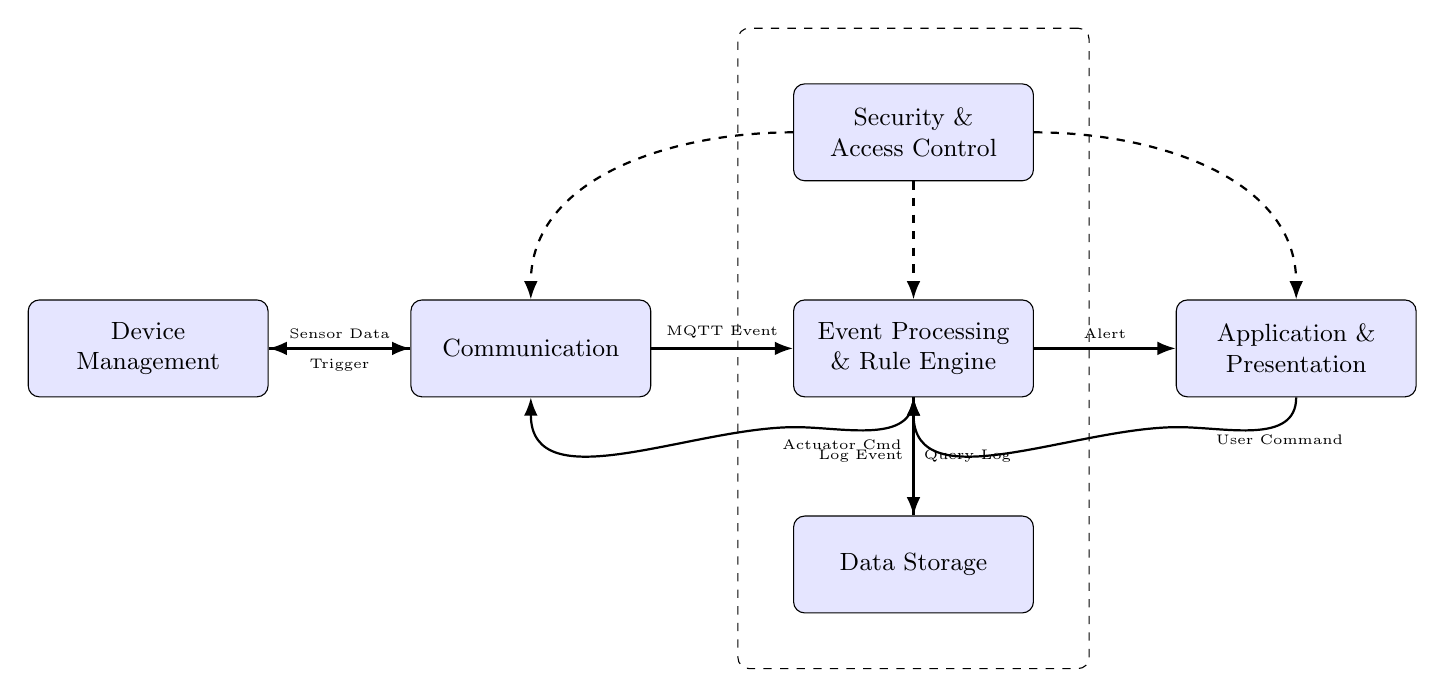
\begin{tikzpicture}[
    node distance=2cm and 1.8cm,
    block/.style={
        rectangle, 
        draw, 
        fill=blue!10, 
        text width=8em, 
        text centered, 
        rounded corners, 
        minimum height=3.5em,
        font=\small
    },
    cloud/.style={
        rectangle,
        draw,
        dashed,
        inner sep=0.7cm,
        rounded corners
    },
    arrow/.style={-Latex, thick},
    label/.style={font=\tiny, text centered}
]

% Main nodes
\node[block] (device) {Device\\Management};
\node[block, right=of device] (comm) {Communication};
\node[block, right=of comm] (processing) {Event Processing\\{\&} Rule Engine};
\node[block, right=of processing] (app) {Application {\&}\\Presentation};

% Cloud components
\node[block, above=1.5cm of processing] (security) {Security {\&}\\Access Control};
\node[block, below=1.5cm of processing] (storage) {Data Storage};

% Cloud boundary
\node[cloud, fit=(processing) (storage) (security), 
      label={[yshift=0.3cm, font=\normalsize]above:Cloud Backend}] (cloud_boundary) {};

% Main data flow arrows
\draw[arrow] (device) -- node[above, label] {Sensor Data} (comm);
\draw[arrow] (comm) -- node[above, label] {MQTT Event} (processing);
\draw[arrow] (processing) -- node[above, label] {Alert} (app);

% Return path
\draw[arrow] (app) to[out=270, in=0] node[below, label, pos=0.3] {User Command} +(-1.5,-1) to[out=180, in=270] (processing);
\draw[arrow] (processing) to[out=270, in=0] node[below, label, pos=0.7] {Actuator Cmd} +(-1.5,-1) to[out=180, in=270] (comm);
\draw[arrow] (comm) -- node[below, label] {Trigger} (device);

% Storage interactions
\draw[arrow] (processing) -- node[left, label] {Log Event} (storage);
\draw[arrow] (storage) -- node[right, label] {Query Log} (processing);

% Security interactions
\draw[arrow, dashed] (security) -- (processing);
\draw[arrow, dashed] (security) to[out=0, in=90] (app);
\draw[arrow, dashed] (security) to[out=180, in=90] (comm);

\end{tikzpicture}
}
\caption{Functional view block diagram showing interactions.}
\label{fig:functional_view}
\end{figure}

A typical intrusion scenario unfolds as follows:
\begin{enumerate}
    \item A sensor (e.g., PIR motion sensor) detects an event. The \textbf{Device Management} block captures this raw signal.
    \item The signal is passed to the \textbf{Communication} block, which formats it into a JSON payload and transmits it securely via MQTT to the cloud.
    \item The \textbf{Event Processing \& Rule Engine} receives the message. The \textbf{Security \& Access Control} block first validates the device's credentials.
    \item The Rule Engine processes the event. It checks the system's state (e.g., "Armed") and decides the event is a valid intrusion.
    \item It issues two commands: first, it instructs the \textbf{Data Storage Management} block to log the event details (sensor ID, timestamp, etc.).
    \item Second, it generates an alert payload and sends it to the \textbf{Application \& Presentation} block via the Communication block's push notification service.
    \item The user receives the alert on their mobile app. They can use the app to send a command back (e.g., "activate siren"). This command flows from the Application block, through Processing, Communication, and finally to the actuator in the Device Management block.
\end{enumerate}
This decoupled architecture ensures that each block can be developed, tested, and scaled independently, creating a robust and maintainable system.




% --- STEP 8 ---
\subsection{Step 8: Operational View Specification}
The operational view outlines the non-functional aspects of the system, focusing on how it will run, maintain itself, and perform under real-world conditions. This section details the key considerations for performance, reliability, and security to ensure the system is not only functional but also robust and trustworthy \cite{wang_iot_devices_security_2024, design_implementation_smart_home_IoT_2024, article_S266729522100026X}.

\subsubsection{Performance and Scalability}
Performance is critical for a security system where response time directly impacts effectiveness.

\begin{itemize}
    \item \textbf{Latency:} The end-to-end latency, from sensor event detection to user notification delivery, is targeted to be under two seconds. This is achieved by:
    \begin{itemize}
        \item Using lightweight communication protocols (MQTT) with low overhead.
        \item Employing an edge-processing model at the IoT hub to filter non-critical events locally.
        \item Leveraging a scalable, low-latency cloud backend with efficient rule processing and push notification services (e.g., APNS, FCM).
    \end{itemize}
    
    \item \textbf{Throughput:} The system is designed to handle concurrent events from multiple sensors without performance degradation. The cloud backend's message broker (e.g., AWS IoT Core) is capable of ingesting millions of messages per second, ensuring that event storms (e.g., multiple doors opening during a break-in) are processed in parallel.
    
    \item \textbf{Scalability:} The architecture is designed to scale horizontally. As users add more devices, the cloud infrastructure can automatically provision more resources (e.g., via auto-scaling groups or serverless functions). The use of a topic-based messaging system (MQTT) allows for the seamless addition of new sensors and zones without reconfiguring the entire system.
\end{itemize}

\subsubsection{Reliability and Availability}
The system must be highly reliable, as downtime could result in a critical security lapse.

\begin{itemize}
    \item \textbf{Device Reliability:} Battery-powered sensors will use low-power protocols like Zigbee to maximize lifespan. The system will implement a health monitoring mechanism where each device periodically sends a "heartbeat" signal. The mobile application will alert the user of low battery levels or if a device goes offline unexpectedly.
    
    \item \textbf{Network Resilience:} In the event of an internet outage, the local IoT hub is designed to operate with degraded functionality. It will still be able to trigger local actuators, such as a siren, based on sensor input. MQTT's Quality of Service (QoS) level 1 will be used for critical messages to ensure "at-least-once" delivery to the cloud broker once connectivity is restored.
    
    \item \textbf{High Availability:} The cloud backend will be deployed on a major cloud provider (e.g., AWS, Azure) with high uptime Service Level Agreements (SLAs), typically 99.9\% or higher. Services will be deployed across multiple availability zones to ensure redundancy and fault tolerance against single-datacenter failures.
    
    \item \textbf{Data Integrity:} Critical data, such as event logs and user settings, will be stored in a replicated database with automated backup procedures to prevent data loss.
\end{itemize}

\subsubsection{Security Considerations}
As a security system, its own digital and physical security is paramount. A multi-layered security approach is adopted:

\begin{itemize}
    \item \textbf{Device Security:} Each IoT device will be provisioned with a unique cryptographic identity (e.g., X.509 certificate) during setup. This ensures that only authenticated and authorized devices can connect to the IoT hub and the cloud backend, preventing device spoofing.
    
    \item \textbf{Communication Security:} All communication channels are encrypted.
    \begin{itemize}
        \item Device-to-hub wireless communication will use protocol-level encryption (e.g., Zigbee's AES-128 or Wi-Fi's WPA3).
        \item Hub-to-cloud and app-to-cloud communication will be encrypted using Transport Layer Security (TLS 1.2+), securing both MQTT and HTTPS traffic against eavesdropping and man-in-the-middle attacks.
    \end{itemize}
    
    \item \textbf{Cloud Security:} The cloud environment will be hardened using the principle of least privilege. Access to resources will be strictly controlled via Identity and Access Management (IAM) roles. Regular security audits and vulnerability scanning will be performed.
    
    \item \textbf{Application and Data Security:} User access to the mobile application will be protected by strong authentication (OAuth 2.0). Support for two-factor authentication (2FA) will be provided. The system will implement Role-Based Access Control (RBAC) to define different permission levels (e.g., Owner, Family Member, Guest). All sensitive data, particularly video recordings, will be encrypted both at rest in cloud storage and in transit.
\end{itemize}

% --- STEP 9 ---
\subsection{Step 9: Device \& Component Integration}
The Smart Home Security System integrates a range of IoT hardware components, each chosen for its reliability, cost-effectiveness, and compatibility with standard IoT protocols. Table~\ref{tab:devices-wide} summarizes the devices and their functions \cite{seerangan_domain_specific_iot_home_automation_2022, tipirisetty_home_automation_case_study_2025, cisco_gateway, cisco_packettracer_iot}.

% preamble once:
\newcolumntype{Y}{>{\raggedright\arraybackslash}X}

\begin{table*}[t]
\centering
\caption{Devices and Components Integration}
\label{tab:devices-wide}
\small
\renewcommand{\arraystretch}{1.25}
\begin{tabularx}{\textwidth}{l Y l l}
\toprule
\textbf{Device/Component} & \textbf{Function} & \textbf{Protocol} & \textbf{Example Model} \\
\midrule
Door/Window sensor & Detects door/window state transitions (open/close) & Zigbee / Wi-Fi & Aqara Contact \\
PIR motion sensor  & Detects human motion via IR changes                 & Zigbee / Wi-Fi & HC-SR501 \\
IP camera          & Streams live video / captures snapshots             & RTSP / Wi-Fi   & ESP32-CAM \\
Siren/Buzzer       & Audible alarm on intrusion                          & GPIO / Zigbee  & Smart Siren Gen5 \\
Smart light        & Illumination deterrent / visual alarm               & Zigbee / Wi-Fi & Philips Hue \\
IoT hub/gateway    & Local aggregation, MQTT client, edge rules          & MQTT / Wi-Fi   & Raspberry Pi 4 \\
Router             & LAN/WAN connectivity                                & Ethernet/Wi-Fi & Cisco 2900 \\
Cloud backend      & Broker, rule engine, storage, notifications         & MQTT / HTTPS   & AWS IoT Core \\
Mobile app         & Status, control, alerts, video                      & HTTPS / MQTT   & Flutter app \\
\bottomrule
\end{tabularx}
\end{table*}



\subsubsection{Integration Architecture}
The integration follows a layered approach:
\begin{itemize}
    \item \textbf{Sensors and Actuators:} Door/window sensors and PIR motion sensors generate real-time status events. Actuators (sirens and lights) receive commands triggered by intrusion events.
    \item \textbf{IoT Hub/Gateway:} A Raspberry Pi acts as the local IoT hub, receiving sensor signals via Zigbee or Wi-Fi. It formats data into lightweight JSON packets and communicates using MQTT.
    \item \textbf{Network Infrastructure:} The hub connects to a Wi-Fi router, ensuring secure internet access for forwarding data to the cloud.
    \item \textbf{Cloud Services:} A cloud backend (e.g., AWS IoT Core) processes events, manages device states, and stores logs and camera feeds.
    \item \textbf{Mobile Application:} The app subscribes to MQTT topics and REST APIs to display alerts, logs, and live video streams to the user.
\end{itemize}




\subsubsection{Communication Flow}
\begin{enumerate}
    \item Sensors detect an event and transmit data to the IoT hub (via Zigbee/Wi-Fi).
    \item The hub authenticates and forwards the event to the cloud service using MQTT over TLS.
    \item The cloud backend triggers a rule engine: it logs the event, sends push notifications, and issues commands to actuators.
    \item Actuators (sirens, lights, cameras) respond immediately to the commands.
    \item The mobile app receives real-time alerts and allows remote control.
\end{enumerate}


\begin{figure}[h]
  \centering
  \resizebox{\columnwidth}{!}{%
  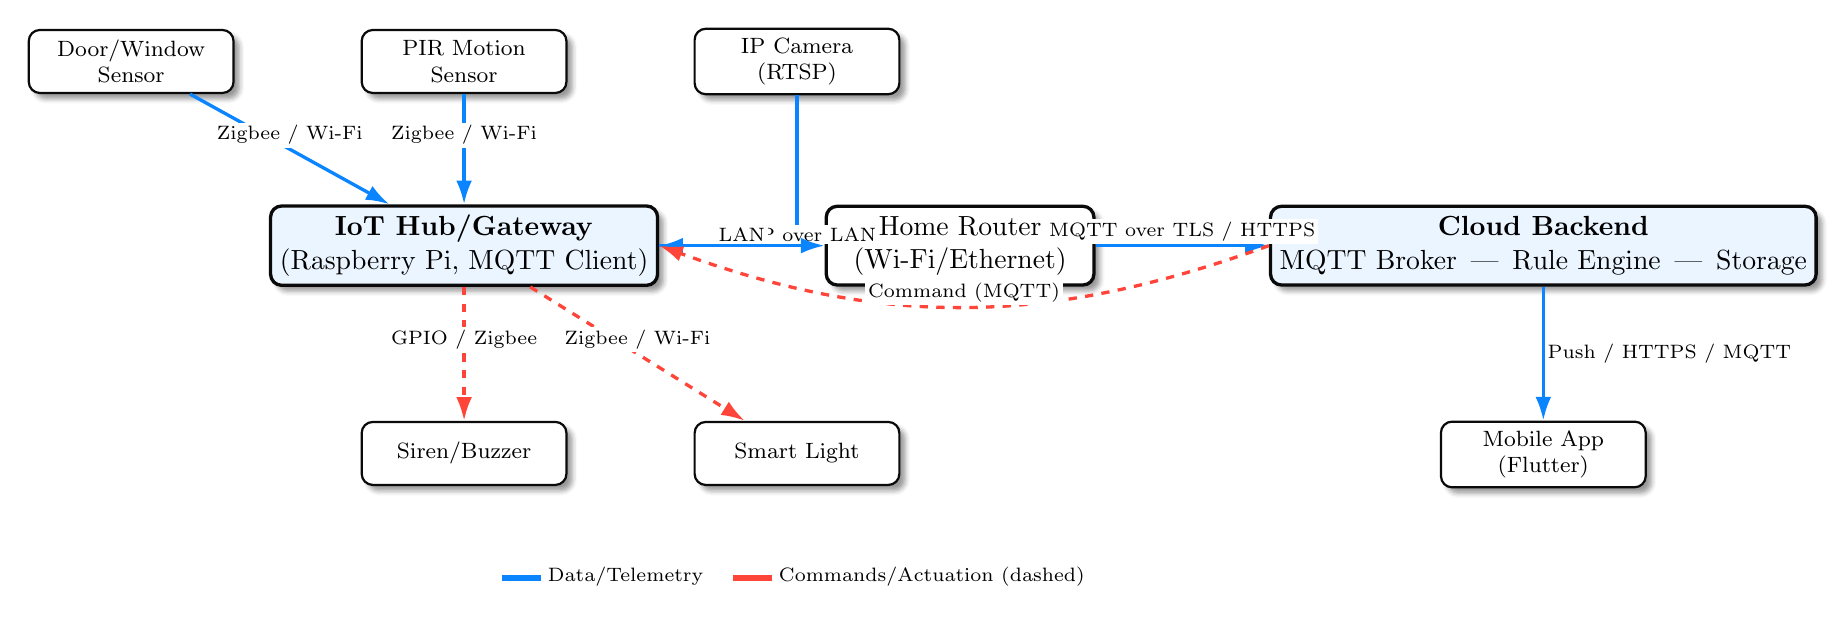
\begin{tikzpicture}[
    node distance=1.2cm and 1.6cm,
    box/.style={rounded corners, draw=ink, very thick, fill=white, blur shadow,
                minimum width=3.4cm, minimum height=1.0cm, align=center},
    small/.style={rounded corners, draw=ink, thick, fill=white, blur shadow,
                  minimum width=2.6cm, minimum height=0.8cm, align=center, font=\footnotesize},
    line/.style={-{Latex[length=3mm,width=2mm]}, very thick, draw=primary},
    cmd/.style={-{Latex[length=3mm,width=2mm]}, very thick, draw=accent, dashed},
    label/.style={font=\scriptsize, midway, fill=white, inner sep=1pt}
  ]

  %%%%%%%%%%%%% Top: Sensors %%%%%%%%%%%%%
  \node[small] (door) {Door/Window\\Sensor};
  \node[small, right=of door] (pir) {PIR Motion\\Sensor};
  \node[small, right=of pir] (cam) {IP Camera\\(RTSP)};

  %%%%%%%%%%%%% Middle-left: Hub & LAN %%%%%%%%%%%%%
  \node[box, below=1.4cm of pir, fill=primary!8] (hub) {\textbf{IoT Hub/Gateway}\\(Raspberry Pi, MQTT Client)};
  \node[box, right=2.1cm of hub] (router) {Home Router\\(Wi-Fi/Ethernet)};

  %%%%%%%%%%%%% Cloud %%%%%%%%%%%%%
  \node[box, right=2.2cm of router, fill=primary!8] (cloud) {\textbf{Cloud Backend}\\MQTT Broker \,|\, Rule Engine \,|\, Storage};

  %%%%%%%%%%%%% Bottom: App & Actuators %%%%%%%%%%%%%
  \node[small, below=1.7cm of cloud] (app) {Mobile App\\(Flutter)};
  \node[small, below=1.7cm of hub] (siren) {Siren/Buzzer};
  \node[small, right=of siren] (light) {Smart Light};

  %%%%%%%%%%%%% Connections: Sensors -> Hub %%%%%%%%%%%%%
  \draw[line] (door) -- (hub) node[label, above] {Zigbee / Wi-Fi};
  \draw[line] (pir) -- (hub) node[label, above] {Zigbee / Wi-Fi};
  \draw[line] (cam) |- (hub) node[label, above] {RTSP over LAN};

  %%%%%%%%%%%%% Hub -> Router -> Cloud %%%%%%%%%%%%%
  \draw[line] (hub) -- (router) node[label, above] {LAN};
  \draw[line] (router) -- (cloud) node[label, above] {MQTT over TLS / HTTPS};

  %%%%%%%%%%%%% Cloud -> App (alerts, control) %%%%%%%%%%%%%
  \draw[line] (cloud) -- (app) node[label, right] {Push / HTTPS / MQTT};

  %%%%%%%%%%%%% Commands back: Cloud -> Hub -> Actuators %%%%%%%%%%%%%
  \draw[cmd] (cloud.west) to[bend left=20] node[label, above] {Command (MQTT)} (hub.east);
  \draw[cmd] (hub) -- (siren) node[label, above] {GPIO / Zigbee};
  \draw[cmd] (hub) -- (light) node[label, above] {Zigbee / Wi-Fi};

  %%%%%%%%%%%%% Legend %%%%%%%%%%%%%
  \node[draw=none, below=0.9cm of light, align=left, font=\scriptsize] (legend) {%
    \textcolor{primary}{\rule{14pt}{2.4pt}}~Data/Telemetry \quad
    \textcolor{accent}{\rule{14pt}{2.4pt}}~Commands/Actuation (dashed)
  };

  \end{tikzpicture}%
  }
  \caption{Device \& Component Integration: sensors stream telemetry to the IoT hub, which relays securely to the cloud; alerts flow to the mobile app, while commands return to local actuators.}
  \label{fig:device_integration_tikz}

\end{figure}
\FloatBarrier


% --- STEP 10 ---
\subsection{Step 10: Application Development}

\subsubsection{Application Overview}
The mobile application provides homeowners with real-time visibility and control over their smart home security system. Core capabilities include device status monitoring, remote control, event notifications, and \textbf{camera integration} for live view and recorded evidence \cite{startertutorials_IoT_methodology, design_implementation_smart_home_IoT_2024, yamini_home_intrusion_2016, sharma_iot_based_smart_home_automation_2020}.

\subsubsection{User Interface (UI)}
The app follows a modern, accessible design (dark/light themes). Primary navigation uses a bottom tab bar: \emph{Home}, \emph{Devices}, \emph{Cameras}, and \emph{Alerts}.

\subsubsection{Main Pages}
\begin{itemize}
  \item \textbf{Home:} System status (Armed/Disarmed), quick actions, and high-level tiles (Door/Window, Motion, Cameras).
  \item \textbf{Door/Window Monitoring:} List of entries with current state (\emph{Open}/\emph{Closed}), and a \emph{View Camera} button for associated zones.
  \item \textbf{Motion Detection:} Zones (e.g., Living Room, Hallway) with \emph{No Motion}/\emph{Motion} state and \emph{View Camera}.
  %\item \textbf{Cameras:} Grid of cameras with \emph{Live} view and \emph{Recordings}. Each camera supports start/stop record and snapshot.
  \item \textbf{Alerts:} Feed of events (icons, time, location) with inline thumbnails and \emph{View Footage}.
\end{itemize}

\FloatBarrier

\subsubsection{UI Flow (Conceptual)}
.
\begin{figure}[h]
  \centering
  \resizebox{\columnwidth}{!}{%
  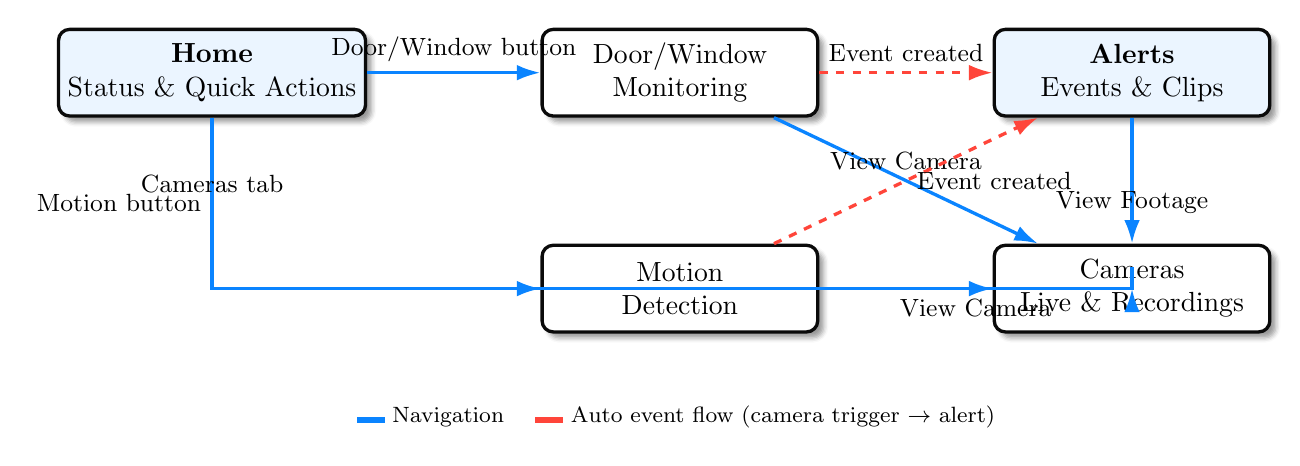
\begin{tikzpicture}[
    node distance=1.6cm and 2.2cm,
    box/.style={rounded corners, draw=ink, very thick, fill=white, blur shadow, minimum width=3.5cm, minimum height=1.1cm, align=center},
    arr/.style={-{Latex[length=3mm,width=2mm]}, very thick, draw=primary}
  ]

  \node[box, fill=primary!8] (home) {\textbf{Home}\\Status \& Quick Actions};
  \node[box, right=of home] (dw) {Door/Window\\Monitoring};
  \node[box, below=of dw] (motion) {Motion\\Detection};
  \node[box, right=of dw, fill=primary!8] (alerts) {\textbf{Alerts}\\Events \& Clips};
  \node[box, below=of alerts] (cameras) {Cameras\\Live \& Recordings};

  \draw[arr] (home) -- node[above]{\small Door/Window button} (dw);
  \draw[arr] (home) |- node[pos=0.25, left]{\small Motion button} (motion);
  \draw[arr] (home) |- node[pos=0.25, above]{\small Cameras tab} (cameras);
  \draw[arr] (dw) -- node[above]{\small View Camera} (cameras);
  \draw[arr] (motion) -| node[pos=0.25, below]{\small View Camera} (cameras);
  \draw[arr, dashed, draw=accent] (dw) -- node[above]{\small Event created} (alerts);
  \draw[arr, dashed, draw=accent] (motion) -- node[right]{\small Event created} (alerts);
  \draw[arr] (alerts) -- node[below]{\small View Footage} (cameras);

  % Legend
  \node[below=0.8cm of motion, align=left] (legend) {\footnotesize
    \textcolor{primary}{\rule{10pt}{2pt}}~Navigation \quad
    \textcolor{accent}{\rule{10pt}{2pt}}~Auto event flow (camera trigger $\rightarrow$ alert)
  };
  \end{tikzpicture}%
  }

  \caption{Navigation and event-driven flow including camera auto-trigger.}
\end{figure}

\FloatBarrier

%\subsubsection{Technical Implementation}
\subsubsection{Platforms}
Cross-platform mobile app using \textbf{Flutter}.

\subsubsection{Communication}
\begin{itemize}
  \item \textbf{MQTT:} Low-latency sensor updates (\texttt{/home/zone1/door}, \texttt{/home/livingroom/motion}).
  \item \textbf{HTTPS REST API:} Event log queries, user actions, and recording retrieval.
  \item \textbf{WebRTC/RTSP:} Live video; recordings stored in cloud object storage.
\end{itemize}

\subsubsection{Backend}
Cloud microservices handle device registry, auth, and event processing. All traffic is encrypted (TLS 1.2+).

\subsubsection{Security}
\begin{itemize}
  \item \textbf{Authentication:} OAuth~2.0 with optional two-factor.
  \item \textbf{Authorization:} Role-based access (Owner, Family, Guest).
  \item \textbf{Privacy:} Encrypted video at rest; signed URLs for clip access; automatic redaction options.
\end{itemize}

\subsubsection{Figures}
App Mockup
\begin{figure}[h]
  \centering
  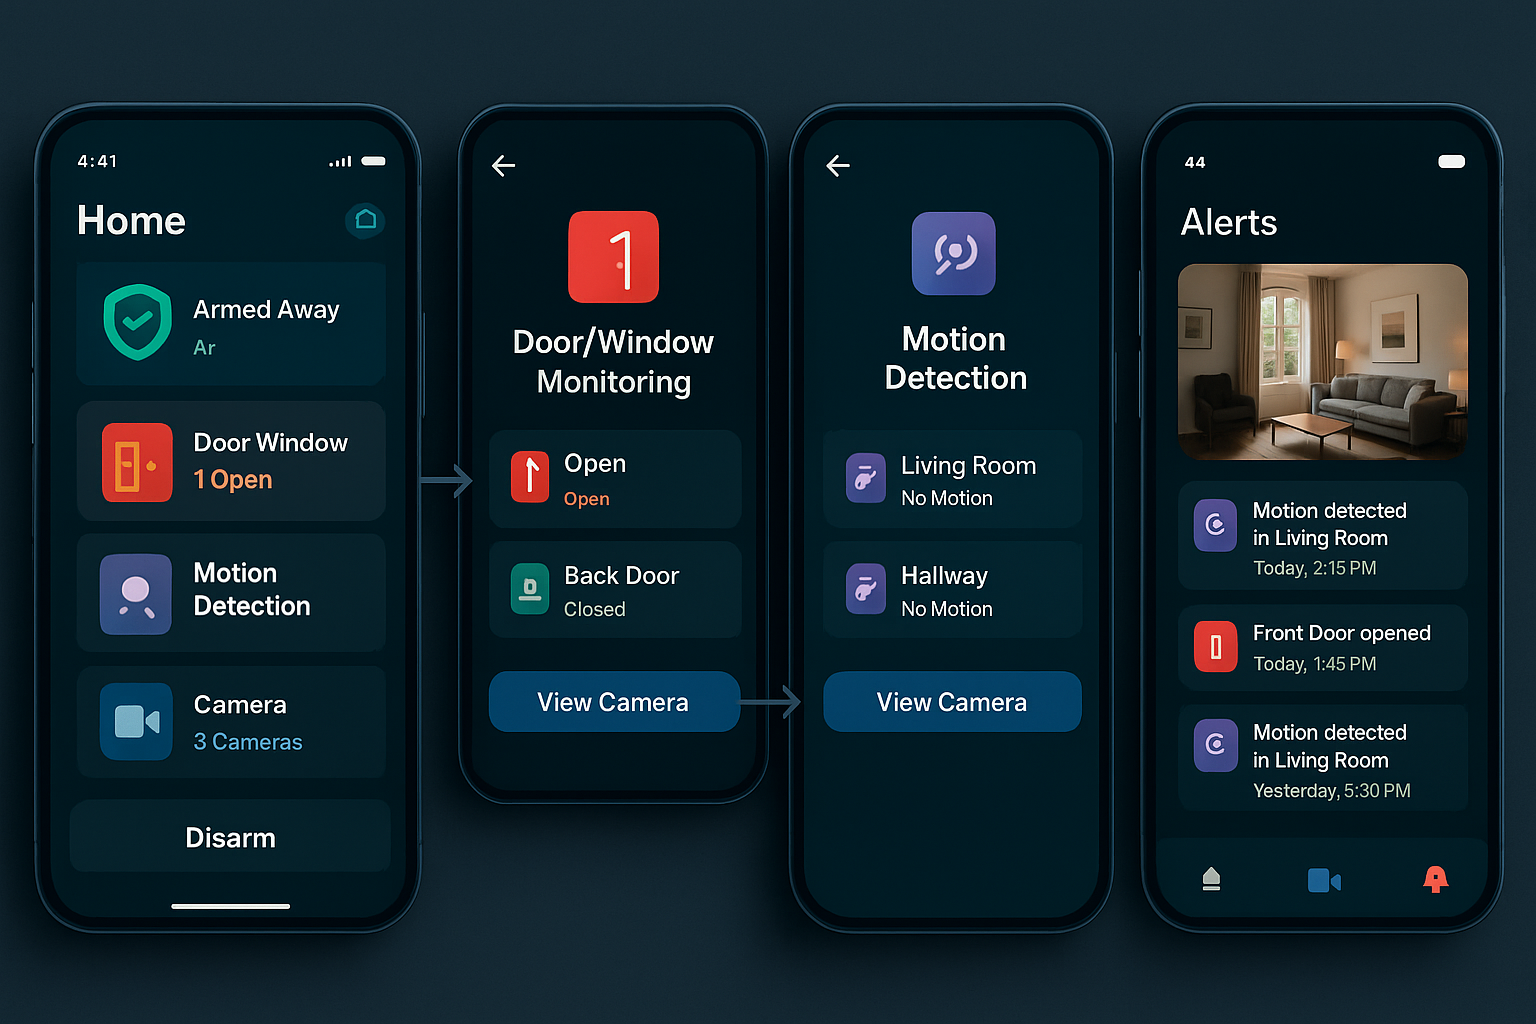
\includegraphics[width=\linewidth]{AppMockup.png}
  \caption{Smart Home Security app mockups showing Home, Door/Window, Motion, and Alerts with camera thumbnails.}
\end{figure}

\FloatBarrier

\subsubsection{Traceability (Features to Screens)}
\begin{center}
\begin{tabularx}{\linewidth}{@{}lX@{}}
\toprule
\textbf{Requirement} & \textbf{UI Location} \\\midrule
Door/Window Monitoring & Home tile; Door/Window page (\emph{View Camera}) \\
Motion Detection & Home tile; Motion page (\emph{View Camera}) \\
Camera Integration & Cameras page; Alerts thumbnails; auto-trigger from events \\
Real-time Alerts & Alerts feed; push notifications \\
Remote Control & Home quick actions; Devices page (Siren/Lights) \\
Monitoring Dashboard & Home overview; Events log on Alerts \\
\bottomrule
\end{tabularx}
\end{center}

% --- Person 5 (HAMSA) writes here ---
% A. Describe the user-facing application (e.g., a mobile app).
% B. Include user interface mockups and describe functionality (dashboard, notifications, etc.).


\section{Conclusion}
This paper has presented a comprehensive blueprint for an IoT-based Smart Home Security System, achieved through the rigorous application of the 10-step IoT design methodology. The resulting design specifies a robust, multi-layered architecture that is secure, scalable, and user-centric. By detailing every stage from requirement analysis and system modeling to component integration and application development, this work establishes a solid foundation for the physical implementation and future enhancement of the system. The proposed design effectively addresses the core challenge of modern home security by creating an intelligent, responsive, and reliable solution.


\section*{Acknowledgment}
Sincere gratitude is extended to Dr. Islam Tharwat Abdel Halim and Eng. Hamdy Osama Mohammed El-Sayed Farag from the Computer and Systems Engineering Department at Ain Shams University for the invaluable guidance, continuous support, and insightful feedback that were provided throughout the course of this project.


%%%%%%%%%%%%%%%%%%%%%%%%%%%%%%%%%%%%%%%%%%%%%%%%%%%%%%%%%%%%%%%%%%%%%%%%%%%%%%%%
% --- BIBLIOGRAPHY SECTION ---
% This tells LaTeX to use the 'IEEEtran' style for references
% and to look for them in the 'references.bib' file.
%%%%%%%%%%%%%%%%%%%%%%%%%%%%%%%%%%%%%%%%%%%%%%%%%%%%%%%%%%%%%%%%%%%%%%%%%%%%%%%%
% \bibliographystyle{IEEEtran}
% \bibliography{references}

\end{document}
